\documentclass[12pt]{article}
\usepackage{amsmath}
\usepackage[margin = 1in]{geometry}
\usepackage{graphicx}
\usepackage{booktabs}
\usepackage{natbib}
\usepackage{lipsum}
\usepackage{setspace}
\usepackage{tikz}
\usepackage{pdfpages}
\usepackage[colorlinks=true, citecolor=blue]{hyperref}
\doublespacing
\title{Machine Learning for Handwriting Recognition: Algorithms and Techniques}
\author{Lai Jiang\\
  University of Connecticut Department of Statistics
}

\begin{document}
\maketitle

\section* {Abstract}
As the topic said, this paper mainly focused on machine learning and handwriting recognition, an area that has grown significantly due to the development of powerful algorithms and sophisticated techniques. It explores the role of machine learning from the basic concepts, data collection methods, data augmentation techniques, and various algorithmic approaches to handwriting recognition, including traditional machine learning and neural networks, a newer way. This article also discusses the impact of machine learning on the connection between human interactions and digital systems, highlighting its potential to improve user experience and facilitate digital interactions. By examining methods and advances in the field, the article reveals the future possibilities and applications of machine learning for accurately and efficiently processing handwritten text.

%\section* {Keywords}
%Machine Learning, Deep Learning, Handwriting Recognition, Activation Function, Model, Parameters...

\section* {Introduction}
In an era where digital communication pervades nearly every facet of our lives, the beauty and uniqueness of human handwriting still holds profound significance. From historical manuscripts to personal notes, handwriting offers a glimpse into a person's individuality and emotions. Yet, decoding diverse handwritten styles and converting them into digital text is a challenging task. The irregularities, variations, and idiosyncrasies present in handwriting have made its recognition one of the most intriguing problems in the realm of pattern recognition and artificial intelligence. However, the evolution of machine learning, with its robust algorithms and sophisticated techniques, has brought groundbreaking advancements to this domain. Handwriting recognition, once a distant dream, is now manifesting in various applications ranging from mail sorting to bank cheque processing and beyond. 

The importance of machine learning in handwriting recognition cannot be overstated, as it stands at the forefront of bridging human interaction with digital systems. This technology plays a crucial role in various applications that significantly impact our daily lives and professional sectors. In the banking industry, it revolutionizes processes by accurately reading handwritten cheques and forms, thus streamlining financial transactions and enhancing security. In the field of education, machine learning algorithms assist in evaluating handwritten exam responses, offering a more efficient grading system while also providing insights into students' learning patterns. Additionally, in historical research, these algorithms are indispensable for digitizing ancient manuscripts and documents, unlocking new realms of knowledge previously inaccessible due to the sheer volume and complexity of handwritten texts. Handwriting recognition also finds its use in personal devices, where it enhances user experience by allowing natural note-taking and communication in users' own handwriting, seamlessly integrating with various languages and scripts. The broad range of these applications not only underscores the versatility and adaptability of machine learning in handwriting recognition but also highlights its potential to transform and facilitate numerous aspects of our digital interactions.This essay delves into the heart of machine learning algorithms and techniques that power handwriting recognition, shedding light on the innovations that bridge the gap between the analog strokes of a pen and the digital bytes of a computer.

\section* {Fundemental Concepts}
So what is machine learning? Basically, machine learning is a subset of the artificial intelligence. It allows systems and software to learn and improve from the dataset or experience from the user without being explicitly programmed. This learning process is driven by algorithms that would interpret and process data, extract patterns and make decisions. In handwriting recognition, the algorithms play a important role in decoding the diversity and complexity of human handwriting. Machine learning can be divided into three main types: supervised learning, where models are trained on labeled data; unsupervised learning, which processes unlabeled data and aims to discover hidden patterns; and reinforcement learning, where models learn through trial and error.Each learning type has a unique impact on handwriting recognition.

In the realm of machine learning, a basic concepts is crucial for advancing applications such as handwriting recognition. And Since handwriting is process of training in machine learning, or more accurately, in deep learning, We need to figure out, the difference between each algorithm, including CNN, RNN and LSTNs, also, we have to deeply distinguish the supervised and unsupervised learning in machine learning field distinctively.

\paragraph{Handwriting Recognition Specifics}
The handwriting is a process of the training in the field of machine learning as well. As a specialized application of machine learning, it entails the intricate process of converting handwritten text into a digital format that machines can understand. This task presents unique challenges due to the vast variability and individuality inherent in human handwriting. Unlike typed text, handwritten characters and words can vary greatly in size, style, alignment, and stroke thickness, even within a single document. Additionally, cursive handwriting introduces complexities such as connected letters and overlapping strokes, making the task of segmentation and recognition notably challenging. In the context of machine learning, these challenges necessitate sophisticated algorithms capable of handling such variability and ambiguity.

There are two primary forms of handwriting recognition exist: offline and online\cite{OF}. Offline recognition involves processing static images of handwritten text, or the image or figure has already been complete, instance like scanned or printed documents and photographs. Under this circumstances, the focus lies in accurately discerning characters and words from a fixed representation, often requiring robust feature extraction and pattern recognition techniques. Online handwriting recognition, in contrast, deals with real-time data. It will translate the words from the scratch that the user made, such as the input from a stylus or digital pen, where the temporal sequence of strokes provides additional context for recognition. This mode can leverage dynamic information like stroke order, pressure, and speed, offering a different dimension of data for machine learning models to analyze.

Futhermore, The sophistication of handwriting recognition systems is further underscored by the need to accommodate diverse handwriting styles, including both print and cursive, as well as the need to be adaptable to multiple languages and scripts, each with its own set of characters and writing rules. Machine learning models in this domain are typically trained on vast data sets containing varied examples of handwriting to enhance their accuracy and generalizability. Pre-processing techniques such as normalization, which adjusts for size and orientation, and noise reduction, which cleans up the image, are crucial steps in preparing the data for these models. The ultimate goal of these systems is to achieve a level of accuracy and efficiency that not only matches human capability but also provides scalable solutions for processing large volumes of handwritten data in various applications, from automated form processing to real-time note translation.

\section* {Data Collection}
When we're dealing with handwriting recognition tasks, choosing the right libraries and packages is crucial to obtain reliable training results. Notable libraries include TensorFlow and Keras, which provide a wealth of deep learning capabilities that are essential for building and training neural networks that can recognize handwritten characters. Additionally, PyTorch is a highly flexible and dynamic open source machine learning framework, particularly known for its easy of using and suitability for a wide range of tasks, including handwriting recognition. It can build, train, and evaluate deep neural networks through a simple Python interface. On the other hand, the MNIST dataset is a classic dataset in the machine learning community, containing 60,000 training images of handwritten digits 0 to 9 and 10,000 test images. Each image is represented in grayscale and is 28 x 28 pixels in size. This dataset has been widely used as a benchmark to evaluate and compare the performance of different algorithms in the field of handwriting recognition. When used in conjunction with PyTorch, the MNIST dataset serves as a powerful tool for efficiently developing and evaluating handwriting recognition models.

\section* {Data Augmentation}
Data augmentation plays a important role in improving the performance of machine learning models in handwriting recognition. Given the inherent variability of human handwriting, robust and diverse datasets are critical for training effective models. Data augmentation involves artificially extending a training data set by creating modified versions of existing data. In handwriting recognition, this can be achieved using various techniques. The most common method is geometric transformation, including rotating, scaling and translating images of handwritten text. This will tell the model to recognize characters and words appearing in different orientations, shapes and sizes. Another technique involves morphological operations such as eroding or stretching text, simulating different writing pressures and line widths. Adding some noise, such as random pixel fluctuations, can also be very beneficial because it prepares the model to handle real-world scenarios where handwritten text may be distorted or unclear.

Data Augmentation also includes a subset, called the Color Space Augmentations. It can be used to adjust the brightness or contrast of the input. These methods are particularly useful for colored ink on the paper. The Elastic distortions would warp the image in a non-linear manner, effectively mimic the natural irregularities in handwriting. Furthermore, synthetic data generation, where entirely new handwriting samples are generated using advanced techniques like Generative Adversarial Networks (GANs), offers a way to significantly expand the dataset, especially in scenarios where data collection is challenging or privacy concerns are paramount. These augmentation techniques not only help in creating a more robust model by providing a wide range of handwriting styles and conditions but also aid in reducing over fitting, ensuring that the model generalizes well to new, unseen data. The strategic use of data augmentation in handwriting recognition thus plays a crucial role in enhancing the accuracy and reliability of the resulting machine learning models.

\section* {Algorithms in Handwriting Recognition}
However, collecting and augmenting the data cannot do everything for us, As I mentioned previously, the MNIST dataset contains 60000 for training purposes and 10000 for optimizing the model, we have to choose a relatively credible approach to recognize what the user have written. For approaches, we now have: Traditional Machine Learning Approaches, Neural Network Approaches and Hybrid. Each of them contains various methods and concepts. The Traditional Machine Learning Approaches is the most fundamental and a little bit of antiquated way. The most well-known of these is the decision tree. 

\begin{itemize}
    \item\textbf{Decision Tree: }The decision tree belongs to the supervised learning and it can tackle classification and regressions tasks. The process of it looks like a flowchart, and each node on the chart contains the "test result" of the event. Decision trees provide an intuitive way to extract decision rules from data. It can be visualized and is easy to understand, even for people without a technical background. At the same time, it also reveals the structure and patterns in the data, helping us understand how decisions are supported by data. For example, Suppose we have a data set about weather conditions and whether outdoor activities are performed, we can setup several parameters to estimate it, such as "Weather", which contains "Sunny, Cloudy, and Raining"; "Temperature", which contains "Hot, Proper, Cold", and the third parameter called "Do we want to do the outdoor activities" which only includes yes or no. Our goal is to create a decision tree that helps us decide whether to engage in outdoor activities based on weather conditions. On the climax of the tree, is "Do we want to do the outdoor activities", then, in the first layer of the tree, are the parameters of the weather "Sunny, Cloudy, and Windy" And after this layer, we can output the decisions with yes or no. In this case, sunny and cloudy, could be "yes", and "no" for the rainy. And after many layers of iteration, it could finally have the ability of predictions.

    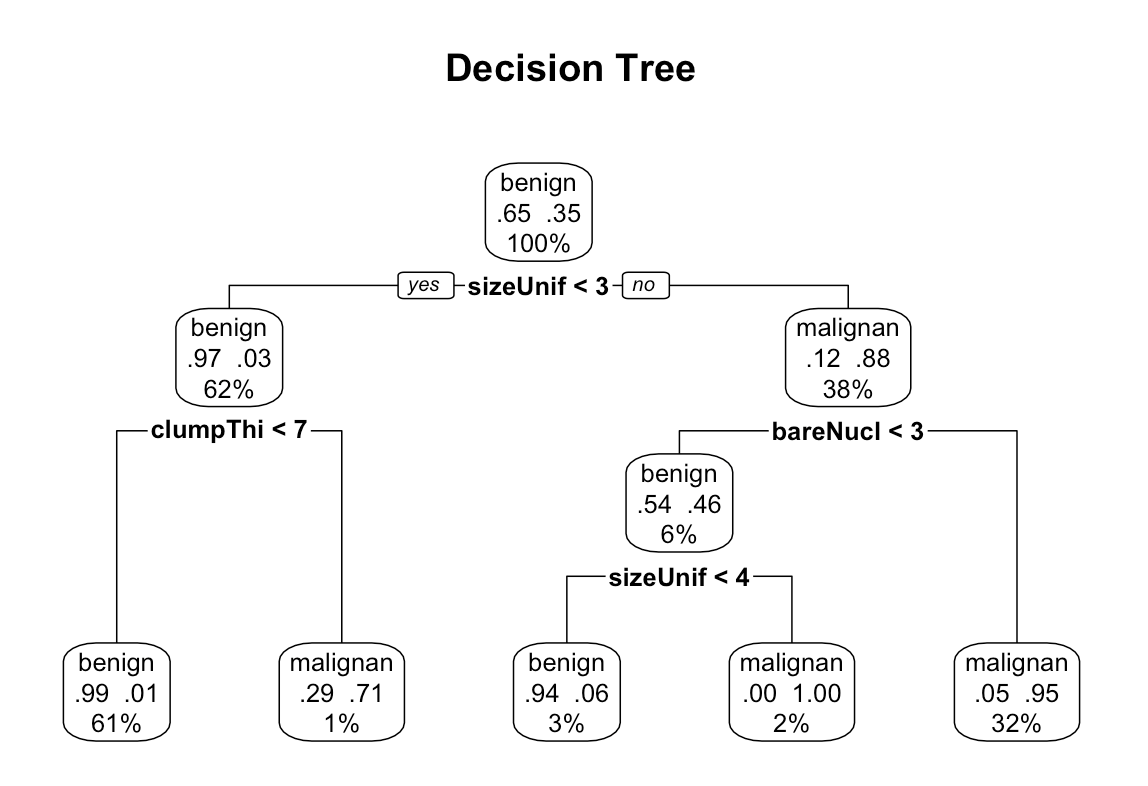
\includegraphics[width = 1.0\textwidth]{Decision Trees.png}
    
    \item \textbf{k-nearest neighbors (KNN)}: KNN is a non-parametric method for classification and regression. It is based on a simple principle, which is predict the label of a point by looking at the "k" closest labeled points and taking a majority vote or average. This method is particularly effective in scenarios with irregular decision boundaries.

    \item \textbf{Support vector machines (SVM)}: SVM is very powerful for classification tasks, especially in high-dimensional spaces. They work by finding the hyperplane that best divides the dataset into categories. The ability of SVM to handle large feature spaces and its effectiveness when the number of dimensions exceeds the number of samples makes it a valuable tool in machine learning.

    \item \textbf{Linear regression}: One of the simplest forms of machine learning, mainly used for regression tasks. The goal is to model the relationship between a dependent variable and one or more independent variables by fitting a linear equation to the observed data. The simplicity of linear regression makes it an excellent starting point for predictive modeling.
\end{itemize}
These traditional methods, although grew up with the development of deep learning and neural networks, it remain integral in scenarios where interpretability, simplicity, and their speed are crucial. They are advantageous in situations with limited data to prevent overfitting and form the backbone of many hybrid approaches, combining strengths of traditional and modern techniques.

\paragraph{Neural Network Approaches}
Although there are many ways to emphasize and implement the machine learning and training process, the most common way that related to neural network could be elaborated like this: For example, if we have a hand-written number, say 7, in this case, how should we let the machine know it is 7? In the MNIST Dataset, all pictures in it are 5 to 5 scaled, which means there are 25 pixels in total. And then we can line them up into a one-dimensional column, and label them 0 if the block or pixel is black, and 1 when this block is white. In order to proceed to the next step, we also need to number them from $X^{0}_{0}$ to $X^{0}_{24}$. The top number refers to the number of layers and the lower number refers to the number of the elements, and in this case, it is refers to every single pixel.Blow is a figure of a complete computing process of handwriting recognition.

\vspace{10pt} 
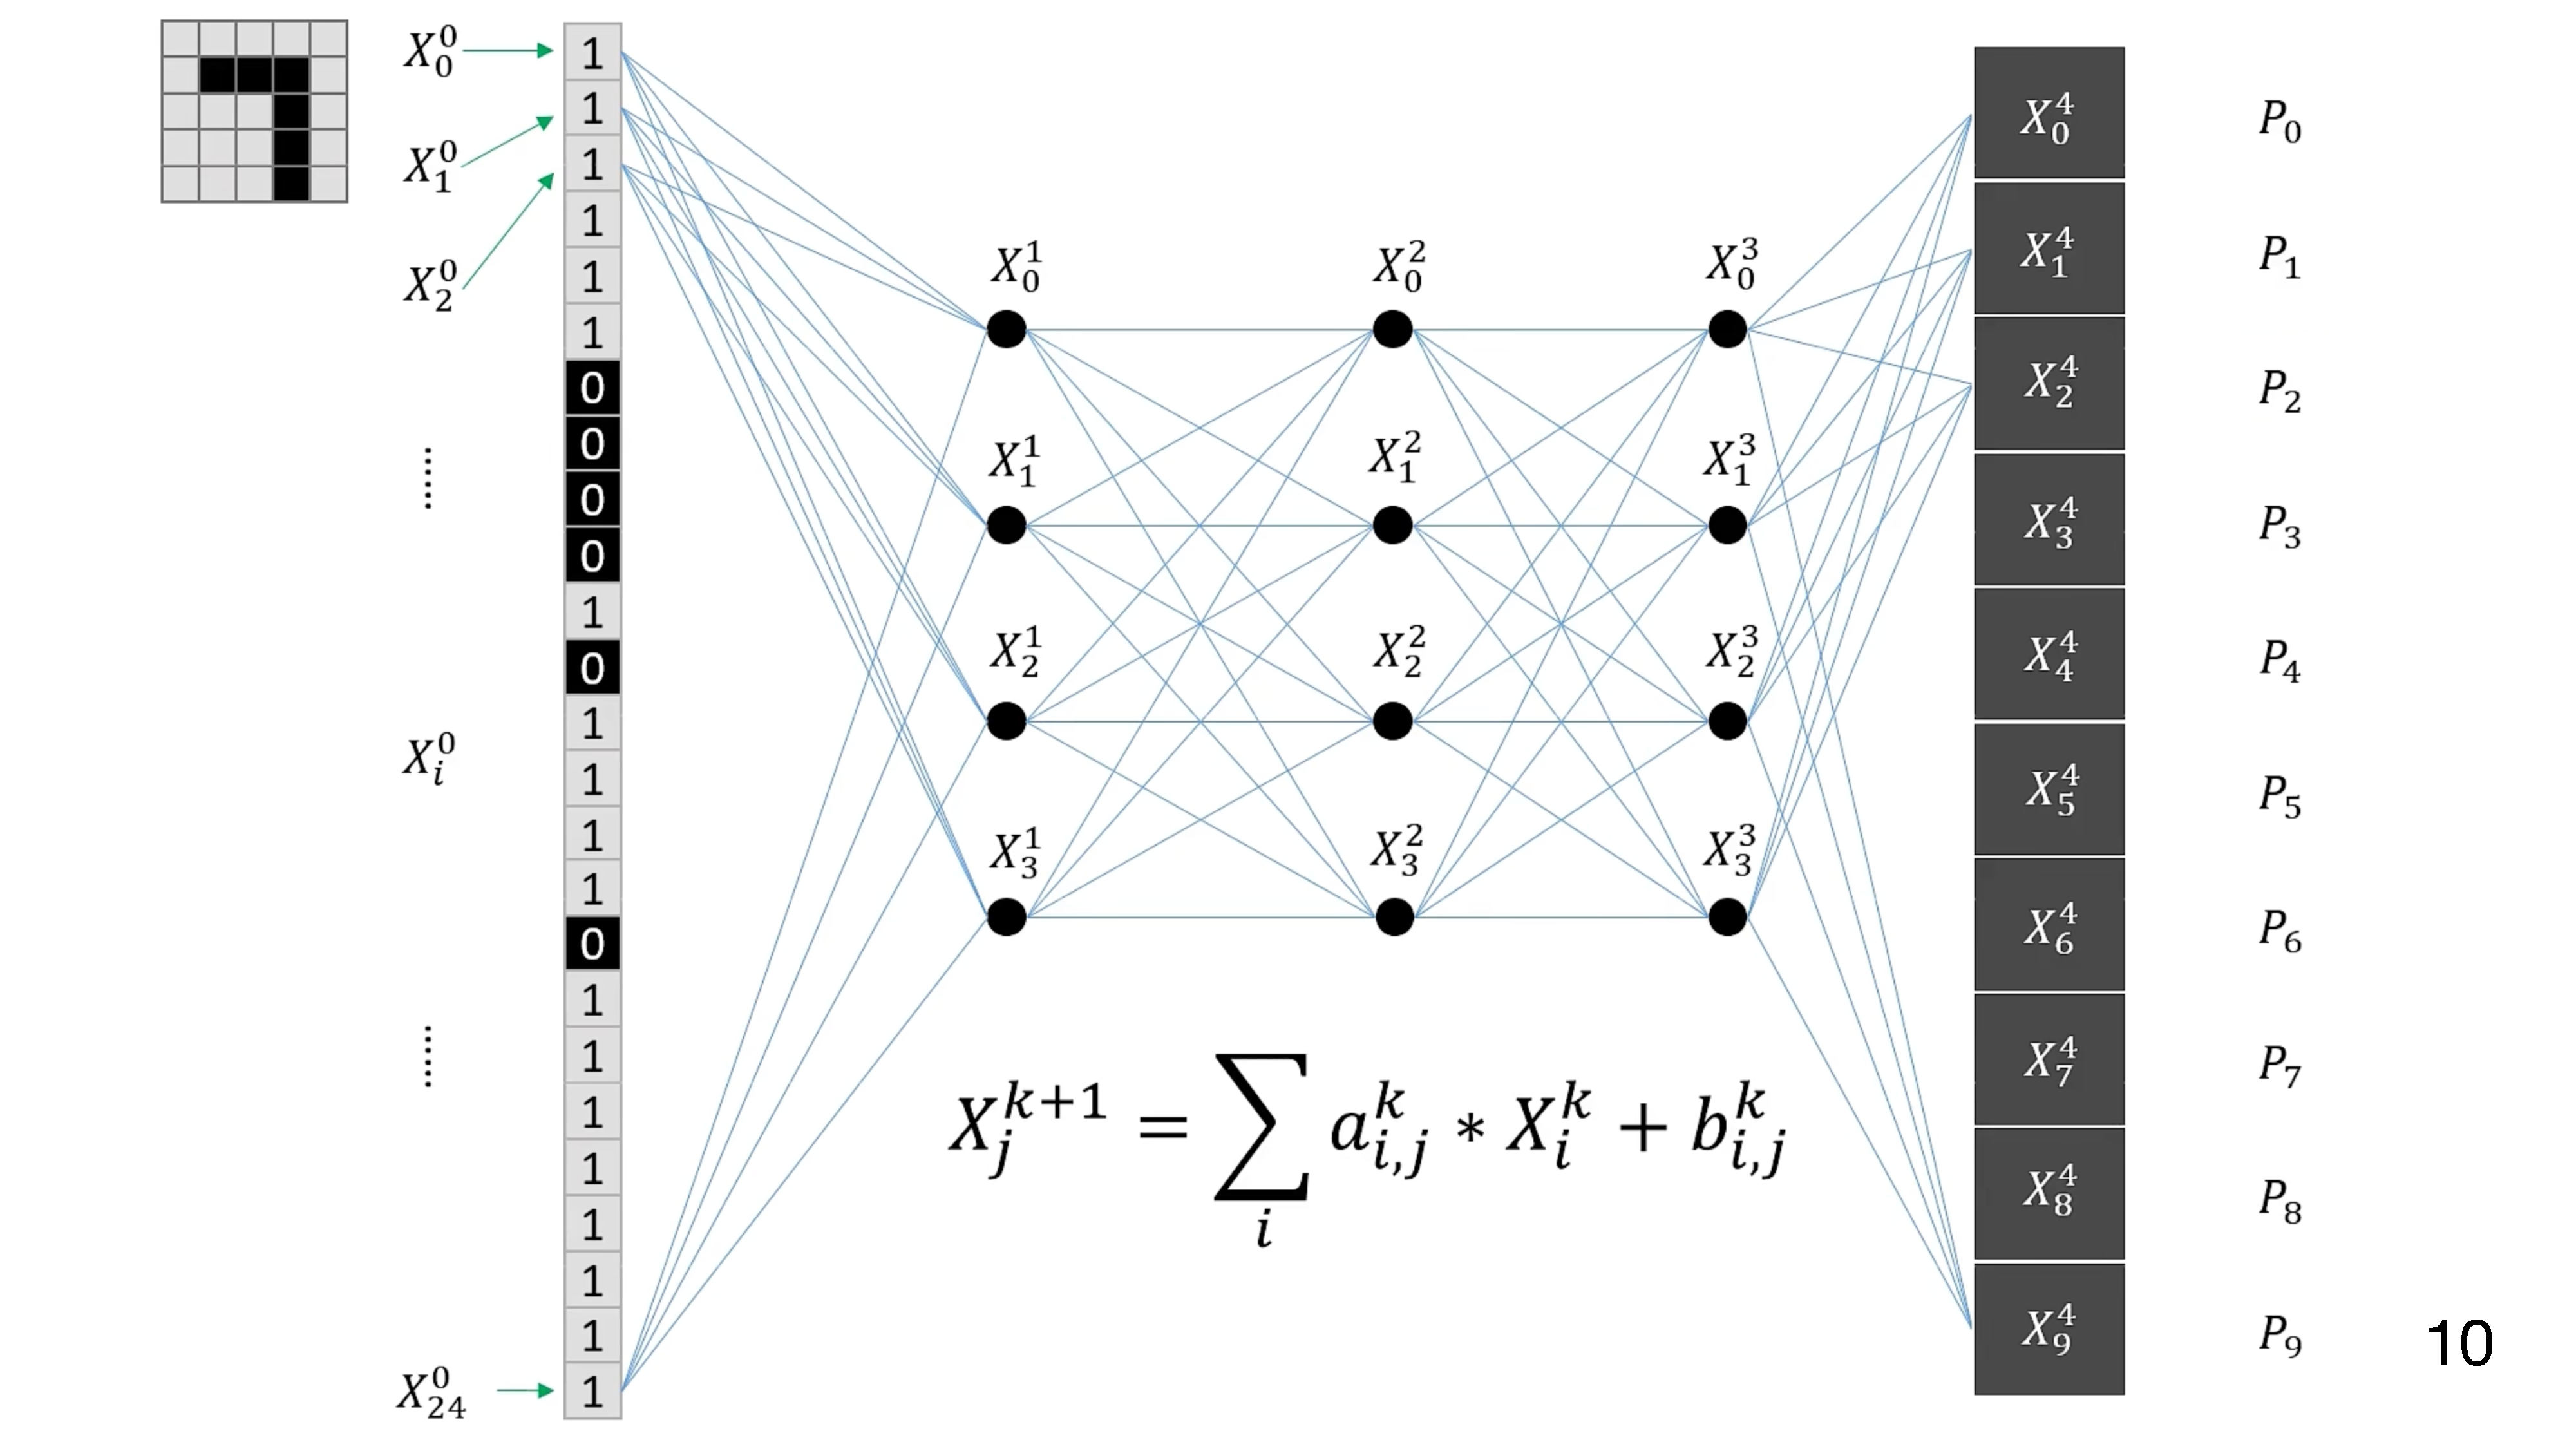
\includegraphics[page = 1, width=\linewidth]{Neural Networks Exemplar.pdf}
Now, the first node in the second layer could be calculated like this: 
\begin{align}
X^1_{0} &= (a^0_{0,0} \times x^0_{0} + b^0_{0,0}) + (a^0_{1,0} \times x^0_{1} + b^0_{1,0}) + \ldots + (a^0_{24,0} \times x^0_{24} + b^0_{24,0}) \\
&= \sum_{i} (a^0_{i,1} \times x^0_{i} + b^0_{i,1})
\end{align}
The letter $a$ and $b$ are the lines here, and the letter i under each X and its parameters refers to the nodes in the previous layer, and the letter j refers to the nodes in the current layer, and similarly, we can also construct the layers of number 2, 3, and 4. And, with the increase of numbers of layers, the formula of the nodes are also extending. The letter k and k+1 refers to the overall layers in this training process, and the parameters, a and b could be arbitrary. The information of the image, spreading across with this formula and finally goes to the last layer of this network. But why there’re 10 results in the final output, the only thing we could image is the probability. This model is to recognize numbers from 0 – 9, so there are only ten possibilities, which just matches the final output. Each output refers to a number. For example, the $P_1$ here refers to the probability of the result is 1. But the parameters between layers, $a$ and $b$ are arbitrary, so, after the calculation from such number of layers, the result should also be arbitrary. Thus, we cannot ensure the probability is from 0 and 1. So, in order to keep the probability is larger than 0, and smaller than 1, we should do some operations. To ensure the probability on the layer of output is larger than 0, smaller than 1 and their sum is 1.

In order to solve this, and let the We will introduce  the mathematical constant to let the probability follow this rule. By putting an e below every X and calculate their values. Therefore, every value will now larger than 0. Then we add them together, then we use the sum as denominator, and we get this formula, the table below shows the relationship.

\begin{table}[h!]
\centering
\resizebox{\textwidth}{!}{% This will scale the table to fit the text width
\begin{tabular}{cccc}
\hline
\( X_0 \) & \( X_1 \) & \(\cdots\) & \( X_n \) \\
\( e^{X_0} \) & \( e^{X_1} \) & \(\cdots\) & \( e^{X_n} \) \\
\( \frac{e^{X_0}}{\sum{e^{X_i}}} \) & \( \frac{e^{X_1}}{\sum{e^{X_i}}} \) & \(\cdots\) & \( \frac{e^{X_n}}{\sum{e^{X_i}}} \) \\
\hline
\end{tabular}
}
\caption{Softmax Normalization}
\label{table:your_label}
\end{table}

As you can see, if we use exponential function first, add them together to obtain a sum, then we use this sum as the denominator, we can get a value between 0 and 1. And this number is what we want. However, if you want these values contain the meaning of probability, or, in other words, "become the probability", you may need to add the activation function. In the example below, the code will show how the activation function works.

\section*{Code Elucidation}
The python file in my Code folder represents an exemplar of the handwriting recognition in machine learning, the purpose of this file is first, we use all the pictures in MNIST Dataset to train and optimize the model, then it will ramdomly extract several pictures from the MNIST Dataset to see its result of prediction, the code was divided into four parts:

Since it is not recommend to insert code clips into this article, readers may refer to the code folder in my repository, and follow the pace of the sections here. So for section one, this is the first paragraph of the code, it defined 5 layers, the first layer fc1 is the input which includes 28 pixels and 64 nodes, and the last layer fc5 contains 10 outputs, and 64 nodes as well. The 64 nodes in layer 2, 3, 4 are used for optimizing and training. And these whole stuff are contained in the "torch.nn.Module" class. 

For section 2, This paragraph just put an ReLu function outside of the layers and that is the activation function of the layer to ensure to produce the real probability. We have a variety of activation functions to choose, including 

In section 3, This paragraph was divided into two parts, the first part just import data from previous layers and make an output as a DataLoader, and the second, The evaluate function is used to estimate the accuracy of the recognition. First, we extract the data from the training set, calculate the accuracy of the neural network, and we compare this value to the Dataset. So these are the normal step of doing such operations in machine learning, especially when training models for handwriting recognition. 

\section*{Discussion}
The complete code is in the GitHub Repository, and when you trying to run it, you may see five epoch will be made in the output, each of them will have a accuracy. For the first epoch, the accuracy is only 11.64 percent, but the second epoch the accuracy goes directly to 95 percent. And for the remaining epoch, the accuracy remains at 97 percent or 96 percent since more training is no longer need to improve accuracy. And you will see five "handwriting pictures" from MNIST Dataset and their predictions. 

\section* {Potential Impact of advancements in handwriting recognition.}
The potential impact of advancements in artificial intelligence and machine learning on handwriting recognition is vast, various and transformative. Because the AI and machine learning technologies continue to evolve, they bring with them the promise of significantly enhancing the accuracy and efficiency of handwriting recognition systems. 

One of the key areas of impact is the improved capability to handle the vast variability in handwriting styles. Advanced machine learning models, especially those employing deep learning techniques like Convolutional Neural Networks (CNNs) and Recurrent Neural Networks (RNNs) we just mentioned above, are becoming increasingly adept at understanding and interpreting the nuances of individual handwriting. This means that as these models are exposed to more data, their ability to accurately recognize even the most idiosyncratic and obscure handwriting styles is greatly enhanced.\cite{Advances}

Another significant impact is the reduction in the need for extensive pre-processing of handwritten texts. Current systems often require multiple steps of pre-processing, such as denoising, normalization, and alignment, to make the text legible for recognition algorithms. However, with advancements in AI, systems are becoming more robust, capable of interpreting text with minimal preprocessing. This not only speeds up the recognition process but also expands the range of applications, enabling the processing of texts in less-than-ideal conditions, such as historical documents or quick handwritten notes.

Additionally, AI advancements are paving the way for real-time handwriting recognition, a feat that was challenging with earlier technologies. This can revolutionize the way we interact with devices, allowing for instantaneous conversion of handwritten notes into digital text, and enabling seamless integration of handwritten input in digital interfaces.

\section* {Challenges in Handwriting Recognition}
Handwriting recognition, although it has significant advancements, it still faces numerous challenges that make its implementation complex and demanding. One of the primary hurdles is the inherent variability in individual handwriting styles. Unlike typed text, which follows a uniform font and spacing, handwritten text varies greatly from person to person. \cite{Improvements}This variability is not just in the shape of the letters, but also in their size, slant, spacing, and the connection between characters. For instance, one individual's 'a' might resemble another's 'o', or the way one person connects letters in cursive writing might be entirely different from another's. This diversity necessitates the development of highly adaptive and sophisticated machine learning models capable of learning and recognizing a wide range of handwriting styles.

Another challenge is handling the skewed, rotated, or poorly scanned text. In real-world applications, the input to handwriting recognition systems can come from various sources. Such as handwritten notes, filled forms, or historical documents, which might not always be perfectly aligned, legible, or well-scanned. Skewed or rotated text requires pre-processing steps for alignment, which can sometimes distort the handwriting, making recognition more difficult. Additionally, the presence of noise, such as smudges, paper quality, or ink blots, can further degrade the quality of the input, posing additional challenges for the recognition algorithms.

\appendix
\section*{Appendix}
The custom software and algorithms developed for this article are available for review and reuse. The source code, along with detailed documentation, is hosted on a GitHub repository.

GitHub Repository Link: https://github.com/statds/course-paper-or-presentation-Bluewiseid.git

This repository includes:

Source code of the developed algorithms.

Be sure to run command "pip/pip3 install torch torchvision numpy matplotlib" before you execute the code.

\bibliographystyle{plain}
\bibliography{Citations.bib}
\cite{Advances}
\cite{Improvements}
\cite{OF}

\end{document}